\section{C-SVM}

\mode<presentation>{
\begin{frame} 
    \begin{center} \huge
        The C-Support Vector Machine (C-SVM)
    \end{center}
    \begin{center}
    No longer assuming perfect separability + regularizing SVMs 
    \end{center}
\end{frame}
}

\begin{frame}\frametitle{Classification of non-separable problems}
	\begin{minipage}{12cm}
		\begin{minipage}{6cm}
			\begin{itemize}
				\item  real-world problems are typically non-separable
				\vspace{1mm}
				\item incomplete feature sets \& noise
				\vspace{1mm}
				\item perfect separation of the training set $\leadsto$ overfitting
			\end{itemize}
		\end{minipage}
		\hfill
		\begin{minipage}{4.5cm}
			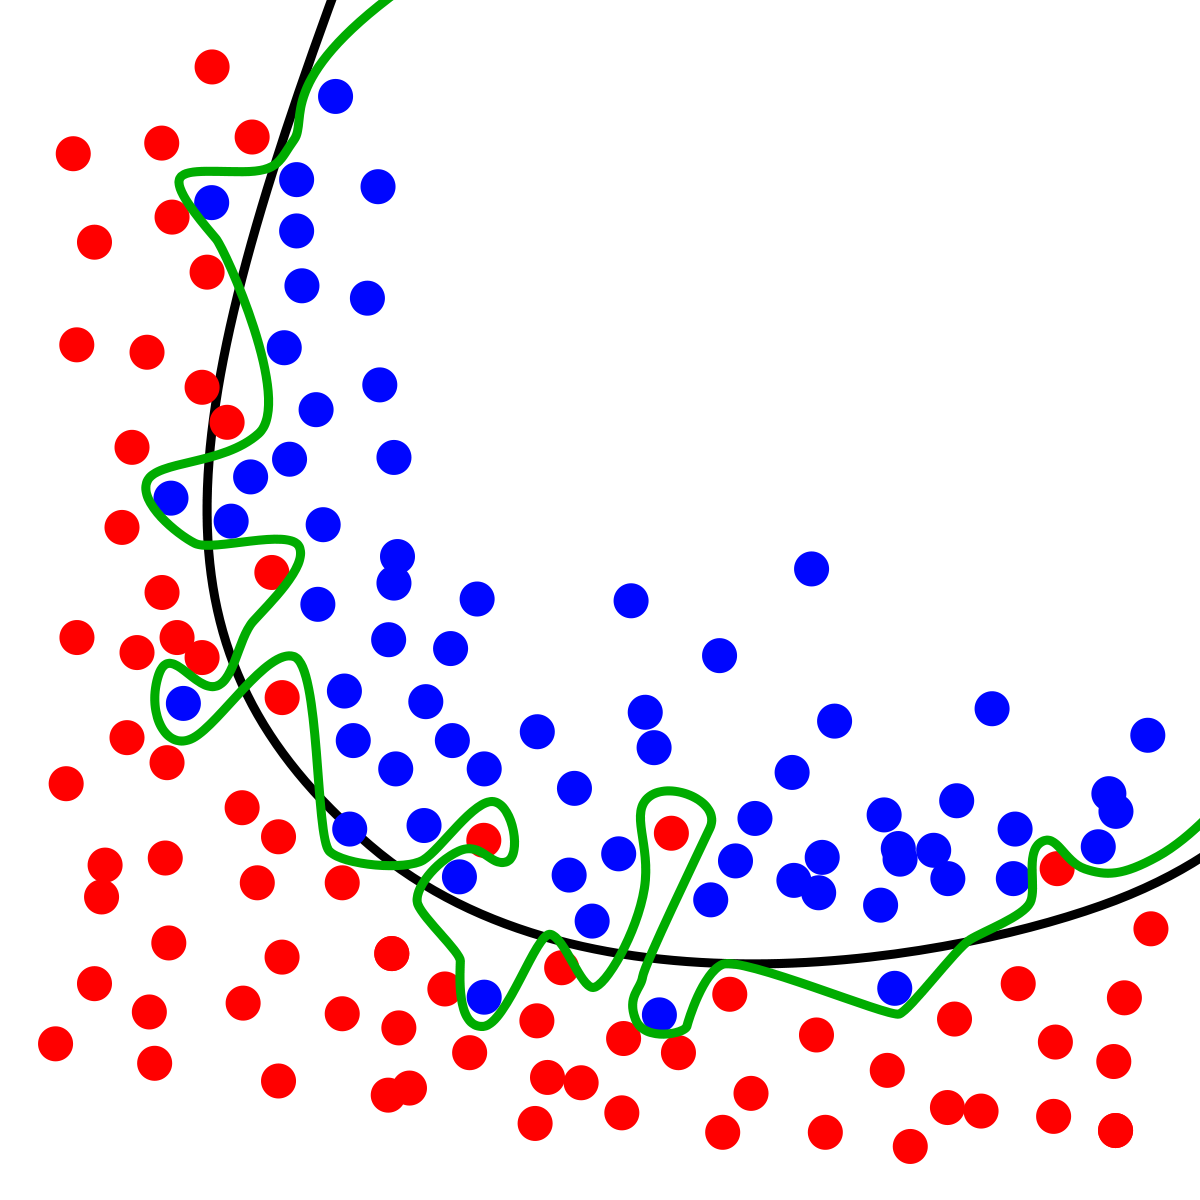
\includegraphics[height=3.5cm]{img/overfitting-classification.png}
		\end{minipage}
	\end{minipage}
	
	\pause

	\begin{block}{consequences}
		$$
			R_{[\vec w]} \quad\leq\quad 
			R_{\emp [\vec w]}^{(p)} \;\;+\;\; C(p,\dvc)
		$$
		\vspace{-3mm}
		\begin{itemize}
			\item finite training error $R_{\emp}^{(p)} \neq 0$ 
			\item trade-off between the minimization of the training error \\
		  		and the capacity of the model class.\\
		  		\slidesonly{Remember weight decay and LASSO regularization?}
		  		
		  		\notesonly{This is similar to the trade-off when regularizing connectionist neurons with weight decay or LASSO regularization. We no longer assume that minimizing the training error is representative of a good solution, particularly in terms of generalizing to unseen data.}
		\end{itemize}
	\end{block}
\end{frame}

\subsection{From hard-margin to the soft-margin hyperplane}


% -----------------------------------------------------------------------------
\begin{frame}\frametitle{\subsecname}

\underline{Hard-margin SVM}:

The margin we were constructing for the SVM so far is considered a ``hard'' in that it prohibits:
\begin{enumerate}
\item miasclassification error, points falling on the \emph{wrong} side of the decision boundary,\\

and

\item points falling \emph{inside} the margin.
\end{enumerate}

This was formulated using the $0-1$ loss as the constraint:

\begin{equation}
y_T^{(\alpha)} \Big( \vec{w}^\top \vec{x}^{(\alpha)} + b \Big)
				\geq 1
\end{equation}

\begin{figure}[h]
	\centering
	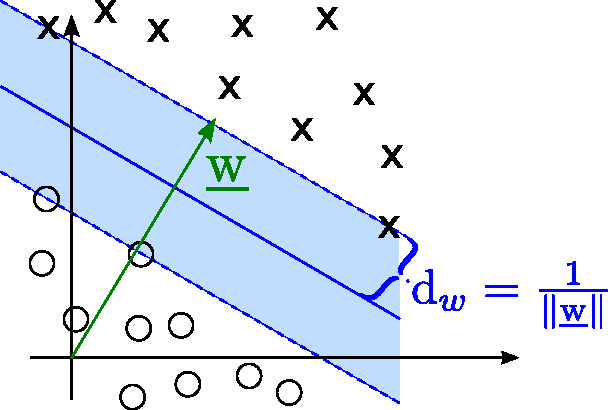
\includegraphics[height=3cm]{img/margin_and_weights}%
	\notesonly{
	\caption{
	Hard margin classification.
	}%
	}%
    \label{fig:marginhard}%
\end{figure}

\end{frame}

\begin{frame}\frametitle{\subsecname}

\underline{Soft-margin SVM (C-SVM)}:

Relaxing the constraint allows for a violating the ``rules'' of the hard margin classifier to a certain extent, which can be controlled.
This is done by introducing a free parameter to the constraint, namely the slack variables $\{\varphi_{\alpha}\}$.
The value of every $\varphi_{\alpha}$ is representative of the margin error.

\begin{equation}
y_T^{(\alpha)} \Big( \vec{w}^\top \vec{x}^{(\alpha)} + b \Big)
				\geq 1 -~{\color{red}\varphi_{\alpha}}
\end{equation}

with $\varphi_{\alpha} \ge 0$.

\begin{figure}[h]
	\centering
	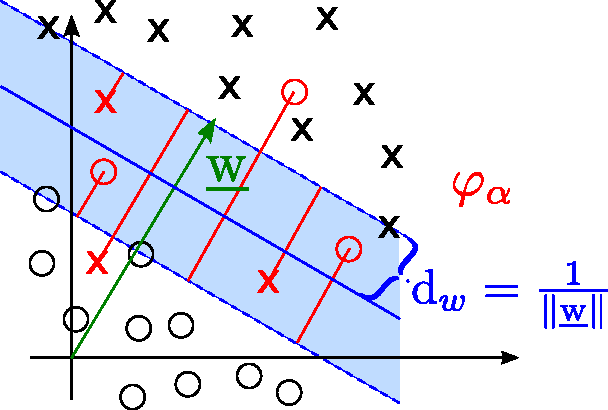
\includegraphics[height=3cm]{img/margin_errors}%
	\notesonly{
	\caption{
	soft-margin classification.
	}%
	}%
    \label{fig:marginsoft}%
\end{figure}

\end{frame}


\subsubsection{The slack values}

\begin{frame}\frametitle{\subsubsecname~: Example}
% Please add the following required packages to your document preamble:
% \usepackage[table,xcdraw]{xcolor}
% If you use beamer only pass "xcolor=table" option, i.e. \documentclass[xcolor=table]{beamer}

\begin{table}[h]
\notesonly{\hskip-2.0cm}% shift table to the left
\resizebox{\textwidth}{!}{%
\begin{tabular}{cccclc}
\begin{tabular}[c]{@{}c@{}}Where is\\ the point\\ relative to\\ the margin?\end{tabular} & \begin{tabular}[c]{@{}c@{}}label\\ $y_T$\end{tabular} & \begin{tabular}[c]{@{}c@{}}prediction\\ $\vec w^\top \vec x + b$\end{tabular} & \begin{tabular}[c]{@{}c@{}}correctly\\ classified\end{tabular} & \begin{tabular}[c]{@{}c@{}} $y_T^{(\alpha)} \Big( \vec{w}^\top \vec{x}^{(\alpha)} + b \Big)
				\geq 1 {\color{blue} - \varphi_\alpha}$\end{tabular}      & \begin{tabular}[c]{@{}c@{}}constraint\\ met for\end{tabular}      
\\ \hline
on  & $\mbox{\scriptsize-1}$                                                    & $\mbox{\scriptsize-1}$                                                        & yes                                                             & \mbox{\scriptsize$-1\cdot(-1) \ge 1-\varphi_\alpha$}        & \mbox{\scriptsize$\varphi_\alpha=0$}
\\ \hline
outside  & $\mbox{\scriptsize+1}$                                                    & $\mbox{\scriptsize-2}$                                                        & no                                                             & \mbox{\scriptsize$+1\cdot(-2) \ge 1-\varphi_\alpha$}        & \mbox{\scriptsize$\varphi_\alpha \ge 3$}
\\ \hline
outside  & $\mbox{\scriptsize+1}$                                                    & $\mbox{\scriptsize+20}$                                                        & yes                                                             & \mbox{\scriptsize$+1\cdot(20) \ge 1-\varphi_\alpha$}        & \mbox{\scriptsize $\varphi_\alpha \ge -19 \Rightarrow$ no slack}
\\ \hline
on  & $\mbox{\scriptsize+1}$                                                    & $\mbox{\scriptsize-1}$                                                        & no                                                             & \mbox{\scriptsize$+1\cdot(-1) \ge 1-\varphi_\alpha$}        & \mbox{\scriptsize$\varphi_\alpha \ge 2$}
\\ \hline
inside  & $\mbox{\scriptsize+1}$                                                    & $\mbox{\scriptsize-0.1}$                                                        & no                                                             & \mbox{\scriptsize$+1\cdot(-0.1) \ge 1-\varphi_\alpha$}        & \mbox{\scriptsize$\varphi_\alpha \ge 1.1$}
\\ \hline
inside  & $\mbox{\scriptsize+1}$                                                    & $\mbox{\scriptsize+0.001}$                                                        & yes                                                             & \mbox{\scriptsize$+1\cdot(0.001) \ge 1-\varphi_\alpha$}        & \mbox{\scriptsize$\varphi_\alpha \ge 0.999$}
\\ \hline
inside  & $\mbox{\scriptsize+1}$                                                    & $\mbox{\scriptsize+0.8}$                                                        & yes                                                             & \mbox{\scriptsize$+1\cdot(0.8) \ge 1-\varphi_\alpha$}        & \mbox{\scriptsize$\varphi_\alpha \ge 0.2$}
\\ \hline
\end{tabular}
}
\caption{Example cases for the slack values.}
\end{table}
\end{frame}


\begin{frame}\frametitle{\subsubsecname~: Overview}

\begin{figure}[h]
	\centering
	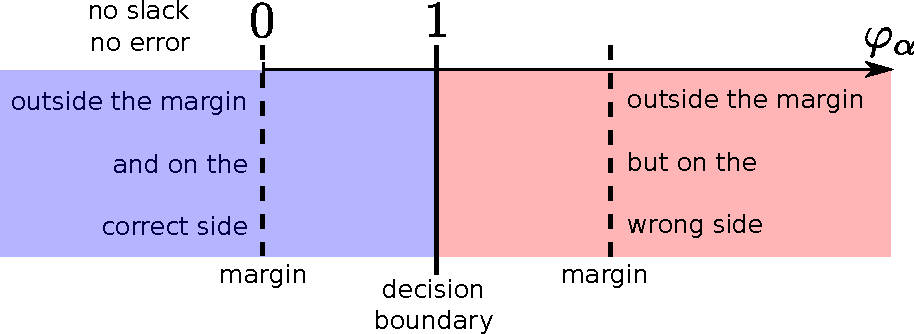
\includegraphics[width=0.6\linewidth]{img/slack_values}%
	\notesonly{
	\caption{
	Overview for interpreting slack values.
	}%
	}%
    \label{fig:unconstrained}%
\end{figure}

\begin{itemize}
\item $0 \le \varphi < 1$:

The data point falls \emph{inside} the margin \textbf{and} on the \emph{correct} side of the decision boundary 


\item $\varphi = 1$:

The data point falls \emph{on} the margin \textbf{and} on the \emph{correct} side of the decision boundary 


\item $\varphi > 1$:

The data point falls on the \emph{wrong} side of the decision boundary. Whether it's \emph{inside}, \emph{outside} or exactly \emph{on} the margin does not matter.

\end{itemize}

\end{frame}


% -----------------------------------------------------------------------------
\begin{frame}
\only<1>{\frametitle{\subsecname~: start with perfect separation - no slack}}
\only<2->{\frametitle{\subsecname~: allow for slack}}

	\slidesonly{\vspace{-5mm}}

	\begin{block}{} 
	\vspace{-4mm}
	\begin{equation}
		\begin{array}{ll}
		\frac{1}{2} \|\vec{w}\|^2 
				\visible<3->{{\color{blue} + \frac{C}{p} 
				\sum\limits_{\alpha = 1}^p \varphi_\alpha}}
			\eqexcl \min \;\;\Bigg\{
		& \begin{array}{l}
			\scriptsize{\text{minimize upper bound on VC dimension}} \\
			\visible<3->{\scriptsize{\text{\color{blue}
				+ minimize (approx.) margin error}}}
		\end{array}
		\end{array}
		\label{eq:csvmmin}
	\end{equation}

	{constraints ($\forall \alpha$):}
	\hfill \only<3>{{{\color{blue}($C > 0$: regularization parameter)}} \normalsize}
	\begin{equation}
		\begin{array}{rll}
			y_T^{(\alpha)} \Big( \vec{w}^\top \vec{x}^{(\alpha)} + b \Big)
				&\geq 1 
				\visible<2->{\color{blue} - \varphi_\alpha}
			& \substack{\text{normalization \& correct classification} \\[1mm]
					\text{of all data points, i.e. ``no slack''}  
					\visible<2->{\color{blue} \text{ for } \varphi_\alpha = 0 } } \\ 
			\visible<2->{\color{blue} \varphi_\alpha & \color{blue} \geq 0 
			& \scriptstyle \color{blue} \text{``margin errors'' for } 
				\varphi_\alpha \neq 0 \text{ ``with slack''}}
		\end{array}
	\end{equation}
	\end{block}
	
	\begin{center}
		\includegraphics<1>[height=3.cm]{img/margin_and_weights}	
		\includegraphics<2,3,4>[height=3.cm]{img/margin_errors}	
	\end{center}
	
	%\begin{itemize}
	%	\itR C: regularization-parameter $\leadsto$ model selection
	%	\itR Why margin error? $\leadsto$ margin necessary for bounding $\dvc$
	%\end{itemize}
	\slidesonly{\vspace{-5mm}}
	
	
	\only<2>{
	\question{What do different values for ${\color{blue}\varphi_\alpha}$ represent?}\\
	}
	
	\only<3>{
	\question{Why do we have to add the ${\color{blue}C}$ term?}\\
	}
	
	\mode<article>{
	Adding The second term to the minimization objective in \eqref{eq:csvmmin} avoids finding the trivial solution where the constrained can be satisifed by making any the slack variable of any point arbitrarily large.
	}
	
	\only<4>{
	\question{How does ${\color{blue}C}$ control complexity?}\\
	}
	
\end{frame}

% ----------------------------------------------------------------------------
\begin{frame}\frametitle{The dual problem of the C-SVM}

	\begin{itemize}
	\item Objective
		\begin{equation}
			-\frac{1}{2} \sum\limits_{\alpha,\beta = 1}^p \lambda_\alpha
				\lambda_\beta y_T^{(\alpha)} y_T^{(\beta)} 
				\underbrace{ \Big( \vec{x}^{(\alpha)} \Big)^\top 
					\vec{x}^{(\beta)}}_{\text{kernel function}}
				+ \sum\limits_{\alpha = 1}^p \lambda_\alpha 
				\quad \eqexcl \quad \max_{\{\lambda_\alpha\}_{\alpha=1}^p}
		\end{equation}
		
		\notesonly{
		See \sectionref{sec:dualtoprimal} for the derivation. The Lagrangian of the dual problem is the same for SVMs and C-SVMs. However,
		the difference is in the constraints.
		}
	%\vspace{3mm}
	\item Constraints:
		\begin{equation}
			\sum\limits_{\alpha = 1}^p \lambda_\alpha y_T^{(\alpha)} = 0 \qquad \text{and} \qquad
			0 \leq \underbrace{\lambda_\alpha 
				\;\;{\color{blue}\leq \frac{C}{p}} }_{
				\substack{ \color{blue} \text{difference to} \\
					\color{blue} \text{separable case}}} 
		\end{equation}
	\end{itemize}
	\mode<presentation>{
	\vspace{-5mm}
	\begin{center}
		\includegraphics<2>[height=3.cm]{img/margin_errors}	
	\end{center}
	}
\end{frame}

% -----------------------------------------------------------------------------
\begin{frame} \frametitle{Margin and support vectors}
	\begin{center} 
		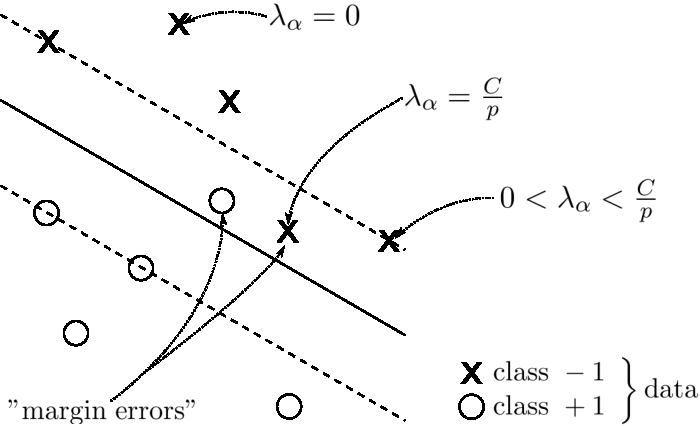
\includegraphics[height=5cm]{img/section2_fig16_v2} 
	\end{center}
	
	\question{Where are the support vectors?}
	
	\pause
	
	\question{Does $C$ influence the number of support vectors?}
	
	
\end{frame}

% -----------------------------------------------------------------------------
\begin{frame}\frametitle{The C-SVM classifier}

SVs do not necessarily lie on the margin anymore. The C-SVM has a ``soft'' margin.

\slidesonly{\vspace{-3mm}}

	\begin{eqnarray*}
		\vec{w} &=& \sum\limits_{\alpha = 1}^p \lambda_\alpha y_T^{(\alpha)}
			\vec{x}^{(\alpha)} \qquad
		\leadsto {\color{red}\lambda_\alpha \neq 0} \text{ only for support vectors }\mathrm{SV}\\[2mm]
		\pause
		b &=& \frac{1}{\# \mathrm{SV}_<} \sum\limits_{\alpha \in \mathrm{SV}_<} \bigg( y_T^{(\alpha)}
			- \sum\limits_{\color{red}\beta \in \mathrm{SV}} \lambda_\beta y_T^{(\beta)} 
			\underbrace{ \Big( \vec{x}^{(\beta)} \Big)^{\kern-0.6ex\top} 
				\kern-0.2ex\vec{x}^{(\alpha)}}_{\text{kernel function}}
			\bigg)
	\end{eqnarray*}
	\vspace{2mm}
	$\mathrm{SV}_<$: $\mathrm{SV}$s with $0 < \lambda_\alpha < \frac{C}{p}$ 
	($\mathrm{SV}$s on the margin) at which $\varphi_\alpha = 0$ (''no slack'').
	
	\notesonly{Further reasoning for why the bias is computed this way is that the bias shifts the hyperplane such that the SVs with zero slack fall on the $\pm1$ lines parallel to the hyperplane.
	}
	
	\pause

	\begin{block}{Classifier}
	\begin{equation*}
		%\hat 
		y(\vec x) = \sign \big( \vec{w}^\top \vec{x} + b \big) 
		= \sign \bigg( \sum\limits_{\alpha \in \mathrm{SV}} \lambda_\alpha y_T^{(\alpha)} 
			\underbrace{ \Big( \vec{x}^{(\alpha)} \Big)^{\kern-0.6ex\top} 
				\kern-0.2ex \vec{x}}_{
				\text{kernel function}} + \;b
			\bigg)
	\end{equation*}
	\end{block}
\end{frame}

\begin{frame}
C-SVM demo: \href{https://cs.stanford.edu/people/karpathy/svmjs/demo/}{Link to C-SVM applet}
\end{frame}
